\subsection{Node Governance} \label{sec:node_governance}
The purpose of Node Governance is to ensure a stable network and that all nodes agrees on the state of the network. The Node Governance is devided into layers of governance as it is defined in \cref{tab:node_governance_layers} and the Node Governance only governances procedures which can be automatomated via algorithms. This section does not inlcude the rules for the user of the network, only the rules for automated nodes. 
\begin{table}[H]
 \begin{center}
  \begin{tabular}{|p{4cm}|p{8cm}|}
   \hline
   Node Layers & Governance Rules \\
   \hline
   Join Layer & Ruling the selection of nodes to join the network. \\
   \hline
   Prospect Layer &  This layer governance the rules to be selected as an node validator. \\
   \hline
   Available Layer & Governance for the validators. \\
   \hline
   Active Layer & Governance the rules of the validators which performs the actual validation work.  \\
   \hline  
  \end{tabular}
 \end{center}
 \caption{The actors in the Tagion Network.}
 \label{tab:node_governance_layers}
\end{table}


A node is defined as an automatomated-unit (computer) which can send/receive information to any other node in a network. The nodes are devided up into node-actors as defined in \cref{tab:node_actors}.
\begin{table}[H]
 \begin{center}
  \begin{tabular}{|p{4cm}|p{8cm}|}
   \hline
   Node Actor & Description \\
   \hline
   External Node \bfit{XN} & Nodes not available for the network.\\
   \hline
   Prospect Node \bfit{PN} & Nodes waiting to become a \bfit{N}. \\
   \hline
   Available Node \bfit{N} & Nodes avliable to be select as a \bfit{RN}. \\
   \hline
   Reserve Node \bfit{RN} & \bfit{PN} are a subset of \bfit{RN}, which are waiting to become a \bfit{AN}. \\
   \hline
   Active Node \bfit{AN} & \bfit{AN} are a subset of \bfit{N}. \bfit{AN} operate and constitute the live Tagion network. \\
   \hline  
  \end{tabular}
 \end{center}
 \caption{The Node actors in the Tagion Network.}
 \label{tab:node_actors}
\end{table}


\begin{figure}[H]
 \centering
 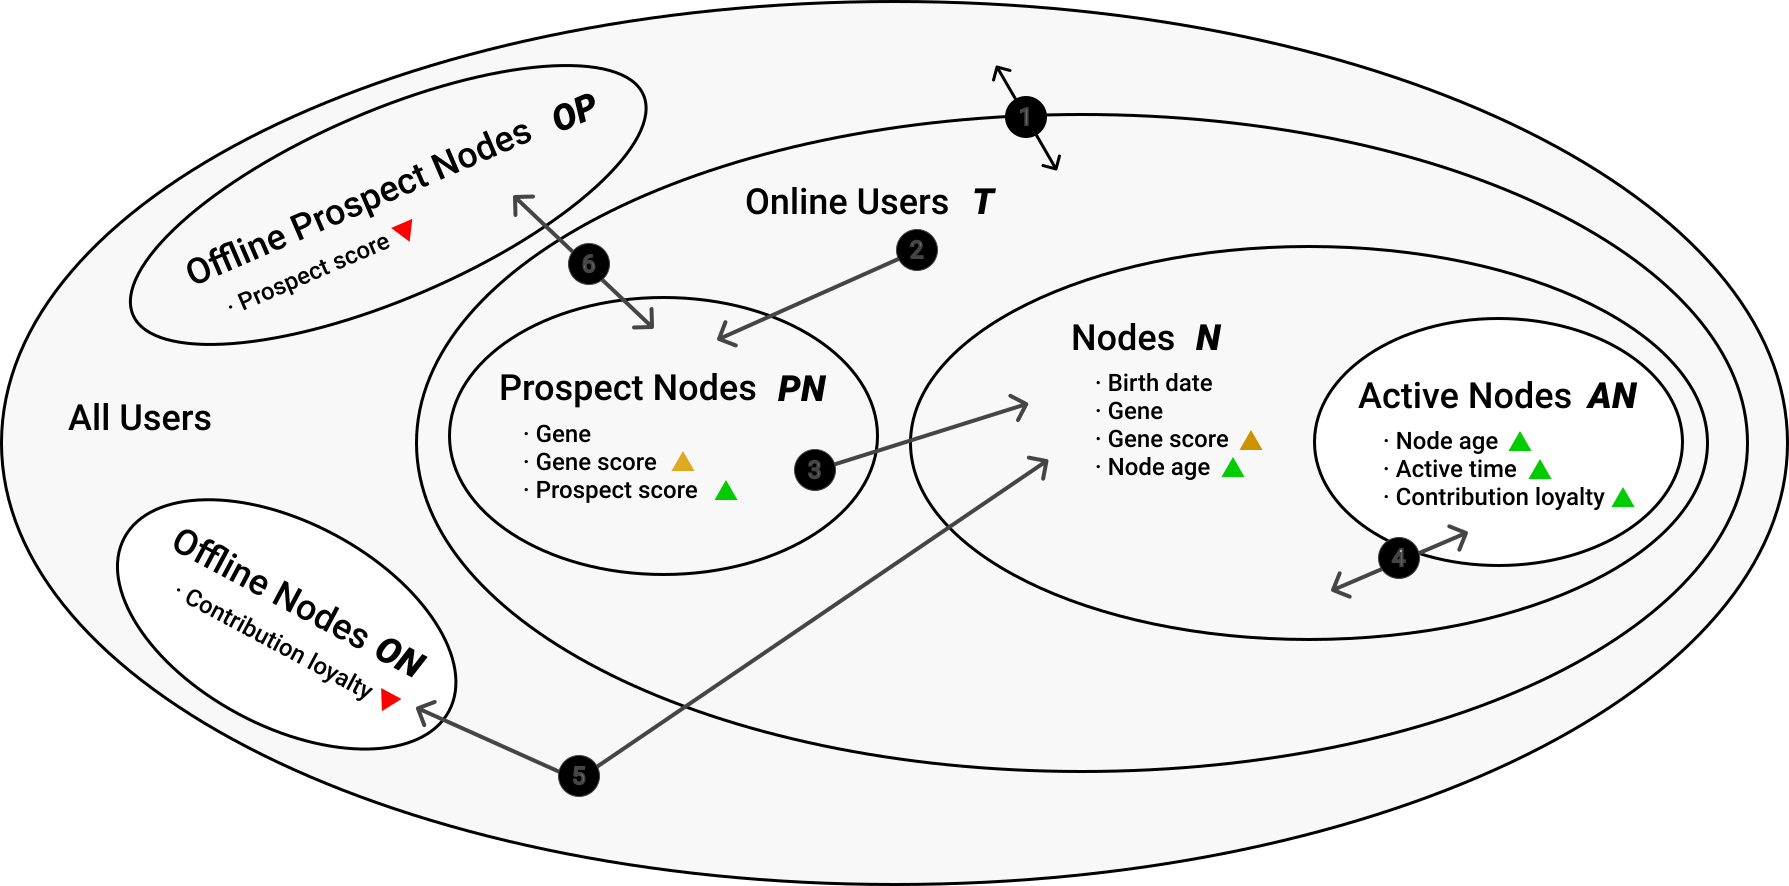
\includegraphics[width=1.05\textwidth]{fig/governance_model.pdf}
 \caption{Governance Model with actors, boundaries and variables in the Tagion system. The green triangle indicates an increase for the actor, the red triangle a decrease and the yellow an increase after an action i.e. a mating transaction.}
 \label{fig:governance_model}
\end{figure}


The boundaries are labelled with numbers in \cref{fig:governance_model} which are defined as:
\begin{enumerate}
 \item Any node can go from online to offline and vice versa. The network is open for all; it means that anyone who has not yet used the system can become a user as well. 
 
 \item Any node can become a validator-node over time and must first become a prospect node. The transition is based on a random selection, a lottery, to help ensure a broad representation of nodes. When going from a user to a prospect node or node, in general, the user is no longer anonymous, but a public servant with a public name record in the system \cref{sec:name_card_contract}.
 
 \item When a prospect nodes have been socially verified and earned enough prospect score that is being available for the network for a period of time then the prospect node becomes a node, i.e. born and receives a gene number and a birth date.
 
 \item Nodes are chosen randomly within a given interval continues to be active nodes, and active nodes are chosen randomly to be inactive nodes. Nodes and active nodes are swapped back and forth continuously to make it impossible to predict, which nodes are active in 10 minute intervals, enhancing security. A node is selected by a \abbrev{UDR}{Unpredictable Deterministic Random} algorithm, where the probability of being chosen as an active node or to continue as an active node depends on four variables:  \abbrev{gs}{Gene score},  \abbrev{at}{active time},  \abbrev{no}{node age} and \abbrev{cl}{contribution loyalty}. 
 \begin{equation}
  P_{(active)} (gs, cl, na/at)
 \end{equation}
 
 \item A node can go from online to offline and vice versa, if offline, it is not possible to be an active node or to become an active node. 
 
 \item A prospect node can go from online to offline and vice versa. 
\end{enumerate}

\subsubsection{External Node Layer} \label{sec:extenal_node_layer}
xxx

\subsubsection{Prospect Node Layer} \label{sec:prostect_node_layer}
xxx

\subsubsection{Available Node Layer} \label{sec:available_node_layer}
xxx

\subsubsection{Active Node Layer} \label{sec:active_node_layer}
xxx


\subsubsection{Reputational Scoring Model} \label{sec:reputational_scoring_model}
The model consists of actors, variables and the boundaries of the actors, including the transition over a boundary.


The variables of the actors and scoring rules for the model are defined in \cref{tab:governance_variables}.
\begin{table}[H]
 \begin{center}
  \begin{tabular}{|p{4cm}|p{8cm}|}
  \hline
  Variable name & Definition and scoring rule \\
  \hline
  Birthdate & The date a prospect node becomes a node. \\
  \hline
  Gene & A gene is unique for each node. \\
  \hline
  Gene score (Gene-diversification points) & Each time a node mates with another node, a score is calculated for them both based on how diverse their genes are compared to each other. They mate each time verification of a prospect node takes place, when an active node makes an epoch, see \cref{sec:hashgraph_cm}, and when two nodes choose to mate and validate each other. \\
  \hline
  Node age & A measure of a node's total available time for the network. Time as both a node and an active node. It increases both as a node and active node when available for the network. \\
  \hline
  Active time & Time as an active node. It increases when a node is active.\\
  \hline
  Prospect score & The Prospect score variable is a measure of how much the prospect node has been available to the network. It increases when the prospect node is available and decreases when not. \\
  \hline
  Contribution loyalty & A measure of how much the node has been active and stayed available. Non-availability of a node decreases contribution loyalty; being an active node increases loyalty. \\
  \hline
  \end{tabular}
 \end{center}
 \caption{Variables and scoring rules for the reputational scoring model}
 \label{tab:governance_variables}
\end{table}


The actors with their boundaries to each other and variables are illustrated in \cref{fig:governance_model}, the boundaries and transition over them are described below.



\subsubsection{Proof-of-People} \label{sec:proof-of-people}
The Proof-of-People protocol is a heuristic protocol with a random and social component. Heuristic, because it aims to secure the democratic principles of one person one node and that it is an actual person behind a node. One person one node cannot be accomplished, but the social component would accomplish an approximation to this. The social component makes it difficult to manage more than one node, and the scoring mechanism makes it less favourable. The approximation would ensure a highly-distributed system when it is combined with a random selection of new prospect nodes. It means no actor or a few actors would control the network when the number of nodes has a certain size, making it secure.

The protocol for becoming a node is:

\begin{enumerate}
 \item A user creates or has a name record in the system, see \cref{sec:name_card_contract}. 
 
 \item A user has a name record with an age of more than one month. The user makes a prospect node record transaction where a node-transaction fee is paid together with a staked amount. The prospect node record contains the user's public key, has the stake attached to it and is linked to the name record.
 
 \item With an average of 10 minutes, a prospect node record is chosen randomly, which burns the stake and gives a node coupon. Then the prospect node should send a proof of activity from within seven days. The proof is simply a public key to a bill in the DART, which are created within the last seven days. 
 
 \item When the user has sent the proof, two random active nodes verify the proof and give a gene to the prospect by crossing their genes with each other. The gene is added to the prospect node record and both parents sign the prospect node record. 
 
 \item \label{itm:mating_transaction} The rewarded node in the same epoch as where the coupon was issued is the first to identify the prospect in a dialogue. If the rewarded node validates the prospect, they make a mating transaction, which both signs. Both nodes receive gene score points for this transaction, and the mating transaction is linked to the prospect node's record. The gene score points are symbolised with the yellow triangle on \cref{fig:governance_model}. 
 
 \item Two semi-determined identifications should be made by two of the next ten epoch rewarded nodes. The prospect engages in a dialogue with potential validators to get two mating transactions. This is the same mating transaction as in \cref{itm:mating_transaction}.
 
 \item Now the node has received three identifications, which means it can start participating as a prospect node on the network, and receive prospect score points. When the node has reached a prospect score threshold the step is completed. 
 
 \item A second semi-determined identification of the prospect is made with two nodes from the last ten epochs from the point the prospect score is reached. This is the same mating transaction as in \cref{itm:mating_transaction}. 
 
 \item The last mating transaction creates a birth date in the prospect node record, making the prospect node a full node on the network. 
\end{enumerate}

There are three main components to the protocol:
\begin{enumerate}
 \item The first selection of prospect nodes introduces a certain time-lag by the need to have a name record with an age of one month and a stake amount. A node transaction fee ensures that small and zero transactions cannot be used to increase the chances of winning the coupon. The fee and stake ensure commitment as well.  
 \item The requirement of activity within the last seven days creates a requirement for the user to have activity in the network. 
 \item A social component that forces new nodes to engage in dialogue with other nodes, thus creating relations and communities. It is a local or virtual identification and dialogue with each other following the protocol. Both parties receive gene score points when mating, thus raising the chance for rewards to create a direct economic incentive and, indirectly, by ensuring non-evil nodes in the system, ensure the long-term sustainability and economic network worth of the system. Therefore, all nodes have a natural incentive to ensure that new nodes are real persons with honest intentions.
\end{enumerate}

A premise for the social protocol to work is that users engage in dialogue; it requires social responsibility and engagement. As long as this premise is true, the node governance components can be adjusted based on the real experience with the test network, where a balance between the work and drag of being and becoming a node compared to actual user adoption and distribution. \newline
Besides the proof-of-people protocol, a continuous evaluation of nodes can be imaged. E.g. each month, all nodes need to engage in dialogue with 3 other nodes receiving gene score points. 
More, the future perspectives of the sharding of the network would allow the network to be more local based, thus removing cultural and language barriers, which can foster people to educate each other and build a culture around the network. 

That is accomplished by a reputational scoring model and a proof-of-people protocol that is a social heuristic protocol. Both components are inspired by Charles Darwin's evolutionary theory of how species best survive in a new environment with the two main elements 1) most diversified paired genes and 2) caretaking of the offspring. These two elements are embedded in the scoring model and protocol. 

\paragraph{Defining a node} is done from democratic principles, where all can participate and where one person has one vote. These principles are translated into a permissionless system where one node has one vote, and where one person only controls one node. It would ensure full distribution of nodes because centralisation is not possible. It is not possible to ensure 100\% that one person can only control one node, but it is the aim. More, it is not required that the network is fully distributed to ensure the network is secure. The requirement is that it is distributed in a way, where many actors control an insignificant amount of nodes, thus avoiding the centralisation of power like in other networks, where few nodes may have majority control. \\
One of the downsides of democracy is that all have the same voting power independent of contribution. Thus, the Tagion system has a scoring system that values loyalty, that is, work through time, but still is open and fair for all to participate. The social component in the proof-of-people protocol tries to ensure that one person only has one node and is a real person. The protocol also selects users randomly to become nodes ensuring even distribution and fairness.  

